\documentclass[12pt]{jsarticle}
\usepackage[dvipdfm,left=1.5cm,right=1.5cm,top=2cm]{geometry}
\usepackage[dvipdfmx]{graphicx}
\usepackage{amsmath, amssymb}
\usepackage{bm}
\usepackage{comment}
\usepackage{framed}
\usepackage{tabularx}
\usepackage{float}
\usepackage{subcaption}
\usepackage{afterpage}
\graphicspath{{image/}}
\setlength{\topmargin}{-1in}
\addtolength{\topmargin}{5mm}
\setlength{\headheight}{5mm}
\setlength{\headsep}{0mm}
\setlength{\textheight}{\paperheight}
\addtolength{\textheight}{-25mm}
\setlength{\footskip}{5mm}

\newcommand{\frontpage}[3]{%
\begin{center}
 \\
\vspace{15em}{\LARGE{}レポート課題}\\
 \\
{\Huge\bf#1}\\
\vspace{30em}
{\LARGE\today}\\
\vspace{2em}
{\LARGE#2 #3}
\end{center}
\thispagestyle{empty}
\clearpage
\setcounter{page}{1}
}

\newcommand{\result}[5]{
\begin{minipage}{0.05\hsize}
(#1)
\end{minipage}
\begin{minipage}{0.22\hsize}
\includegraphics[width=\linewidth]{#2}
\end{minipage}
\begin{minipage}{0.22\hsize}
\includegraphics[width=\linewidth]{#3}
\end{minipage}
\begin{minipage}{0.22\hsize}
\includegraphics[width=\linewidth]{#4}
\end{minipage}
\begin{minipage}{0.22\hsize}
\includegraphics[width=\linewidth]{#5}
\end{minipage}
\\
}

\begin{document}

\frontpage
{自己符号化器の特性評価}
{S152114}
{宮地雄也}

\section{実験目的}

ニューラルネットワークによる生成モデルの基礎となる自己符号化器の原理および特性について理解する.

\section{実験原理}

\subsection{自己符号化器(Autoencoder,AE)}
自己符号化器とは入力に対して同じものを出力するように学習するニューラルネットワークである.
教師なし学習に分類される.


\subsubsection{自己符号化器の構成要素とそれぞれの役割}
Auto Encoderには大きく分けて,エンコーダー部分とデコーダー部分に分かれる.
エンコーダー部分でその特徴量を学習しながらその次元を圧縮し,それを基にデコーダー部分では復元を行う.
そのイメージを以下に示す.
\begin{figure}[ht]
  \begin{center}
    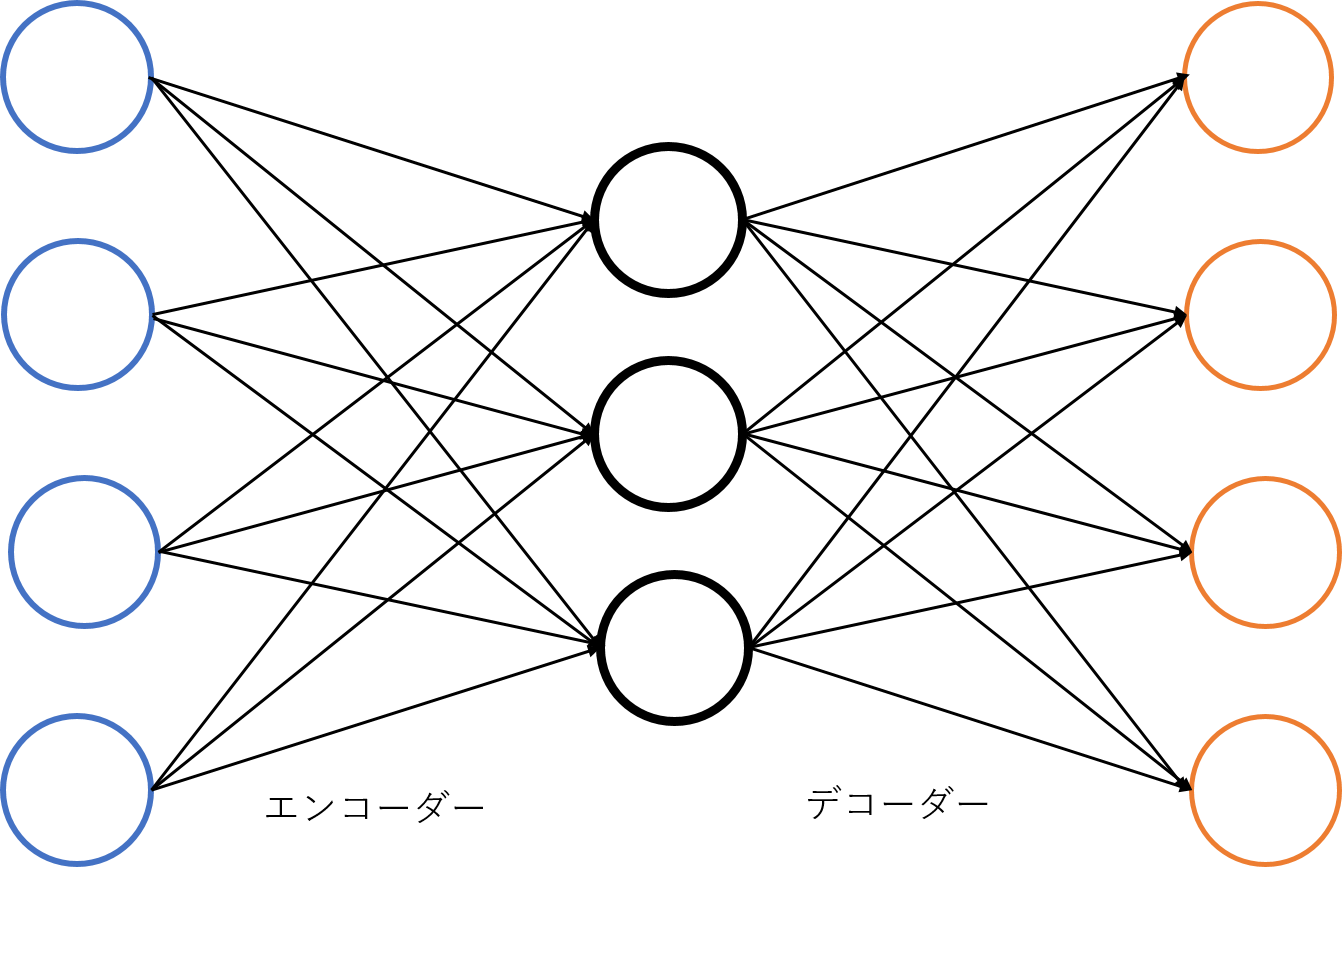
\includegraphics[width = 6cm]{AE_image.png}
  \end{center}
\end{figure}


\subsubsection{主な応用先}
自己符号化器は次元削減や情報検索の分野で応用されてきた.\\
次元削減では自己符号化器で学習したパラメータを深層学習の初期パラメータとして使うことで
多次元のデータも効率よく学習ができ,次元を圧縮してもカテゴリ分類がうまくされていた.
低次元表現は分類問題で効果を発揮し,より効率よくタスクを分類できる.
また消費するメモリーと実行時間も短く出来る.
\\
情報検索とは入力データから似た項目を検索するタスクである.
入力から低次元のバイナリーを作成することで検索を効率化することが出来る.
\\


\subsubsection{学習を成功させるための条件}
学習を成功させるために今回はミニバッチ法を用いる.
ミニバッチ法とは正則化の方法のひとつで,学習時にデータをためてから一気に更新していく手法である.


\subsubsection{主成分分析との関連}
主成分分析(Principle Component Analysis)とは,学習データ$ x_i = (x_i_1,...,x_i_d ) $
の分散が最大になる方向への線形変換を求める手法である.


\subsection{雑音除去自己符号化器(Denoising Autoencoder,DAE)}

雑音除去自己符号化器は破損したデータ点を入力として受け取りもとの破損していないデータ点を復元するよう訓 練された自己複合化器である.
以下にDAEの訓練手順を示す.
\begin{enumerate}
  \item 入力データに一部ノイズを加えたデータをAEを行う
  \item 生成したデータとノイズをつける前のデータの誤差で逆伝播を行う
  \item 繰り返すことでノイズを除去するよう訓練していく
\end{enumerate}

このようにして学習した自己符号化器はノイズを除去するように復元するのでノイズを含んだ学習データから元の綺麗な画像を作り出すことができる

\section{実験方法}

本実験にて確認したいことは以下の2つである。

\begin{itemize}
  \item 画像がきちんとデノイジングされるかどうか
  \item 自己符号化器で学習したパラメータを使うと画像認識にどのような効果があるか
\end{itemize}

この二点について実験を行い、その効果を確認する.
上記のことを確認するために実験は次のように行う.

学習条件
\begin{itemize}
  \item 学習データ:Cifer10
  \item 学習データ数:100枚
  \item 分類テストデータ数:1000枚
  \item 学習回数:500回
  \item パラメーターの初期化方法:ガウス分布でランダムに初期化
  \item パラメータの更新方法:Adamアルゴリズムで更新
  \item ノイズの入れ方:画像の3割から5割をランダムで画素値を0にしてノイズとする
\end{itemize}

今回,実験で利用したネットワーク構成は以下のとおり.\\\\

\begin{table}[ht]
\begin{center}
\caption{オートエンコーダーARAの構成}
\label{table:AE:ARA}
\begin{tabularx}{0.9\linewidth}{|l|l|X|}
\hline
1 & アフィン層 & 入力チャネル数:$3$,入力サイズ:$32 \times 32$,出力チャネル数:$1$,出力サイズ:$500 $ \\
\hline
2 & 検出層 & ReLU \\
\hline
3 & Affine層 & 入力ノード数:$500$,出力チャネル数:$3$, 出力ノード数:$ 32 \times 32 $ \\
\hline
\end{tabularx}
\end{center}
\end{table}

\begin{table}[ht]
\begin{center}
\caption{オートエンコーダーARAAの構成}
\label{table:AE:ARAA}
\begin{tabularx}{0.9\linewidth}{|l|l|X|}
\hline
1 & アフィン層 & 入力チャネル数:$3$,入力サイズ:$32 \times 32$,出力チャネル数:$1$,出力サイズ:$1000 $ \\
\hline
2 & 検出層 & ReLU \\
\hline
3 & Affine層 & 入力ノード数:$500$, 出力ノード数:$ 512 $ \\
\hline
4 & Affine層 & 入力ノード数:$512$,出力チャネル数:$3$, 出力ノード数:$ 32 \times 32 $ \\
\hline
\end{tabularx}
\end{center}
\end{table}

\begin{table}[ht]
\begin{center}
  \caption{オートエンコーダーCRPCRPAAの構成}
\label{table:CRPCRPAA}
\begin{tabularx}{0.9\linewidth}{|l|l|X|}
\hline
1 & 畳み込み層 & 入力チャネル数:$3$,入力サイズ:$32 \times 32$,出力チャネル数:$10$,出力サイズ:$28 \times 28$,カーネルサイズ:$5 \times 5$ \\
\hline
2 & 検出層 & ReLU \\
\hline
3 & プーリング層 & 入力サイズ:$28 \times 28$,出力サイズ:$14 \times 14$,ブロックサイズ:$2 \times 2$,集約演算:最大値 \\
\hline
4 & 畳み込み層 & 入力チャネル数:$10$,入力サイズ:$14 \times 14$,出力チャネル数:$10$,出力サイズ:$10 \times 10$,カーネルサイズ:$5 \times 5$ \\
\hline
5 & 検出層 & ReLU \\
\hline
6 & プーリング層 & 入力サイズ:$10 \times 10$,出力サイズ:$5 \times 5$,ブロックサイズ:$2 \times 2$,集約演算:最大値 \\
\hline
7 & Affine層 & 入力ノード数:$250$,出力ノード数:$500$ \\
\hline
8 & Affine層 & 入力ノード数:$500$,出力チャネル数:$3$,出力ノード数:$ 32 \times 32 $ \\
\hline
\end{tabularx}
\end{center}
\end{table}

\begin{table}[ht]
\begin{center}
\caption{オートエンコーダーCRPCRPAAAの構成}
\label{table:CRPCRPAAA}
\begin{tabularx}{0.9\linewidth}{|l|l|X|}
\hline
1 & 畳み込み層 & 入力チャネル数:$3$,入力サイズ:$32 \times 32$,出力チャネル数:$10$,出力サイズ:$28 \times 28$,カーネルサイズ:$5 \times 5$ \\
\hline
2 & 検出層 & ReLU \\
\hline
3 & プーリング層 & 入力サイズ:$28 \times 28$,出力サイズ:$14 \times 14$,ブロックサイズ:$2 \times 2$,集約演算:最大値 \\
\hline
4 & 畳み込み層 & 入力チャネル数:$10$,入力サイズ:$14 \times 14$,出力チャネル数:$10$,出力サイズ:$10 \times 10$,カーネルサイズ:$5 \times 5$ \\
\hline
5 & 検出層 & ReLU \\
\hline
6 & プーリング層 & 入力サイズ:$10 \times 10$,出力サイズ:$5 \times 5$,ブロックサイズ:$2 \times 2$,集約演算:最大値 \\
\hline
7 & Affine層 & 入力ノード数:$250$,出力ノード数:$500$ \\
\hline
8 & Affine層 & 入力ノード数:$500$,出力ノード数:$512$ \\
\hline
9 & Affine層 & 入力ノード数:$512$,出力チャネル数:$3$,出力ノード数:$ 32 \times 32 $ \\
\hline
\end{tabularx}
\end{center}
\end{table}

\begin{table}[ht]
\begin{center}
\label{table:CCRPACCRPAA}
\caption{オートエンコーダーCCRPACCRPAAの構成}
\begin{tabularx}{0.9\linewidth}{|l|l|X|}
\hline
1 & 畳み込み層 & 入力チャネル数:$3$,入力サイズ:$32 \times 32$,出力チャネル数:$10$,出力サイズ:$29 \times 29$,カーネルサイズ:$4 \times 4$ \\
\hline
2& 畳み込み層 & 入力チャネル数:$10$,入力サイズ:$29 \times 29$,出力チャネル数:$10$,出力サイズ:$26 \times 26$,カーネルサイズ:$4 \times 4$ \\
\hline
3 & 検出層 & ReLU \\
\hline
4 & プーリング層 & 入力サイズ:$26 \times 26$,出力サイズ:$13 \times 13$,ブロックサイズ:$2 \times 2$,集約演算:最大値 \\
\hline
5 & 畳み込み層 & 入力チャネル数:$10$,入力サイズ:$13 \times 13$,出力チャネル数:$10$,出力サイズ:$10 \times 10$,カーネルサイズ:$3 \times 3$ \\
\hline
6 & 畳み込み層 & 入力チャネル数:$10$,入力サイズ:$111 \times 11$,出力チャネル数:$10$,出力サイズ:$10 \times 10$,カーネルサイズ:$2 \times 2$ \\
\hline
7 & 検出層 & ReLU \\
\hline
8 & プーリング層 & 入力サイズ:$10 \times 10$,出力サイズ:$5 \times 5$,ブロックサイズ:$2 \times 2$,集約演算:最大値 \\
\hline
9 & Affine層 & 入力ノード数:$250$, 出力ノード数:$ 500 $ \\
\hline
10 & Affine層 & 入力ノード数:$500$,出力チャネル数:$3$, 出力ノード数:$ 32 \times 32 $ \\
\hline
\end{tabularx}
\end{center}
\end{table}

\begin{table}[ht]
\begin{center}
\label{table:CCRPACCRPAAA}
\caption{オートエンコーダーCCRPACCRPAAAの構成}
\begin{tabularx}{0.9\linewidth}{|l|l|X|}
\hline
1 & 畳み込み層 & 入力チャネル数:$3$,入力サイズ:$32 \times 32$,出力チャネル数:$10$,出力サイズ:$29 \times 29$,カーネルサイズ:$4 \times 4$ \\
\hline
2& 畳み込み層 & 入力チャネル数:$10$,入力サイズ:$29 \times 29$,出力チャネル数:$10$,出力サイズ:$26 \times 26$,カーネルサイズ:$4 \times 4$ \\
\hline
3 & 検出層 & ReLU \\
\hline
4 & プーリング層 & 入力サイズ:$26 \times 26$,出力サイズ:$13 \times 13$,ブロックサイズ:$2 \times 2$,集約演算:最大値 \\
\hline
5 & 畳み込み層 & 入力チャネル数:$10$,入力サイズ:$13 \times 13$,出力チャネル数:$10$,出力サイズ:$10 \times 10$,カーネルサイズ:$3 \times 3$ \\
\hline
6 & 畳み込み層 & 入力チャネル数:$10$,入力サイズ:$111 \times 11$,出力チャネル数:$10$,出力サイズ:$10 \times 10$,カーネルサイズ:$2 \times 2$ \\
\hline
7 & 検出層 & ReLU \\
\hline
8 & プーリング層 & 入力サイズ:$10 \times 10$,出力サイズ:$5 \times 5$,ブロックサイズ:$2 \times 2$,集約演算:最大値 \\
\hline
9 & Affine層 & 入力ノード数:$250$, 出力ノード数:$ 500 $ \\
\hline
10 & Affine層 & 入力ノード数:$500$, 出力ノード数:$ 512 $ \\
\hline
11 & Affine層 & 入力ノード数:$512$,出力チャネル数:$3$, 出力ノード数:$ 32 \times 32 $ \\
\hline
\end{tabularx}
\end{center}
\end{table}


\clearpage

\section{実験結果}

以下のような結果が得られた.

・AE

\begin{figure}[h]
  \begin{center}
    \begin{tabular}{c}

      % 1
      \begin{minipage}{0.43\hsize}
        \begin{center}
          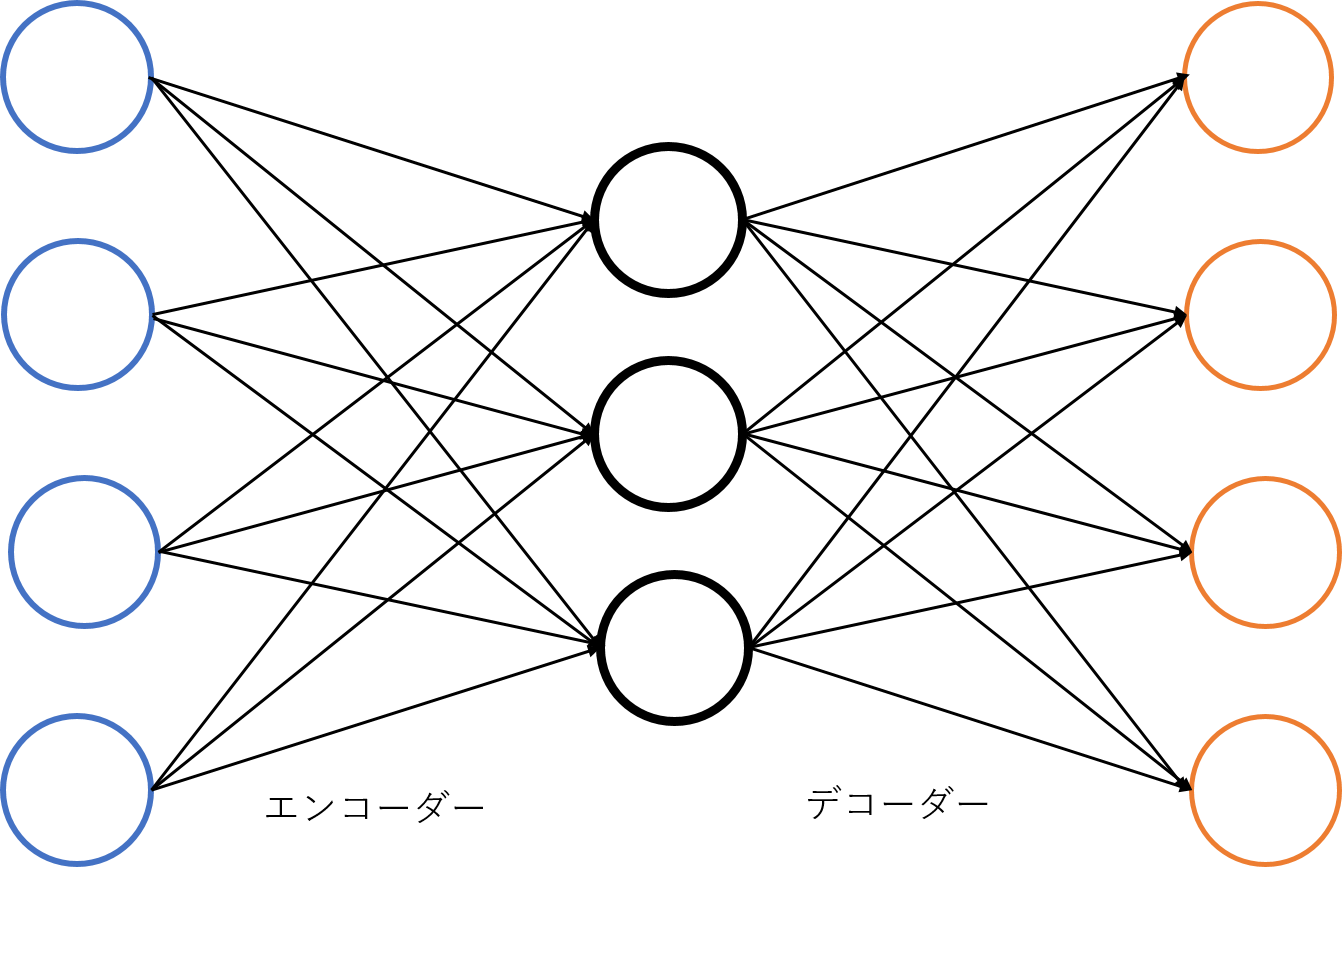
\includegraphics[clip, width=\linewidth]{AE_image.png}
          \hspace{0.2cm} [1]正解率(実験1)
        \end{center}
      \end{minipage}

      % 2
      \begin{minipage}{0.43\hsize}
        \begin{center}
          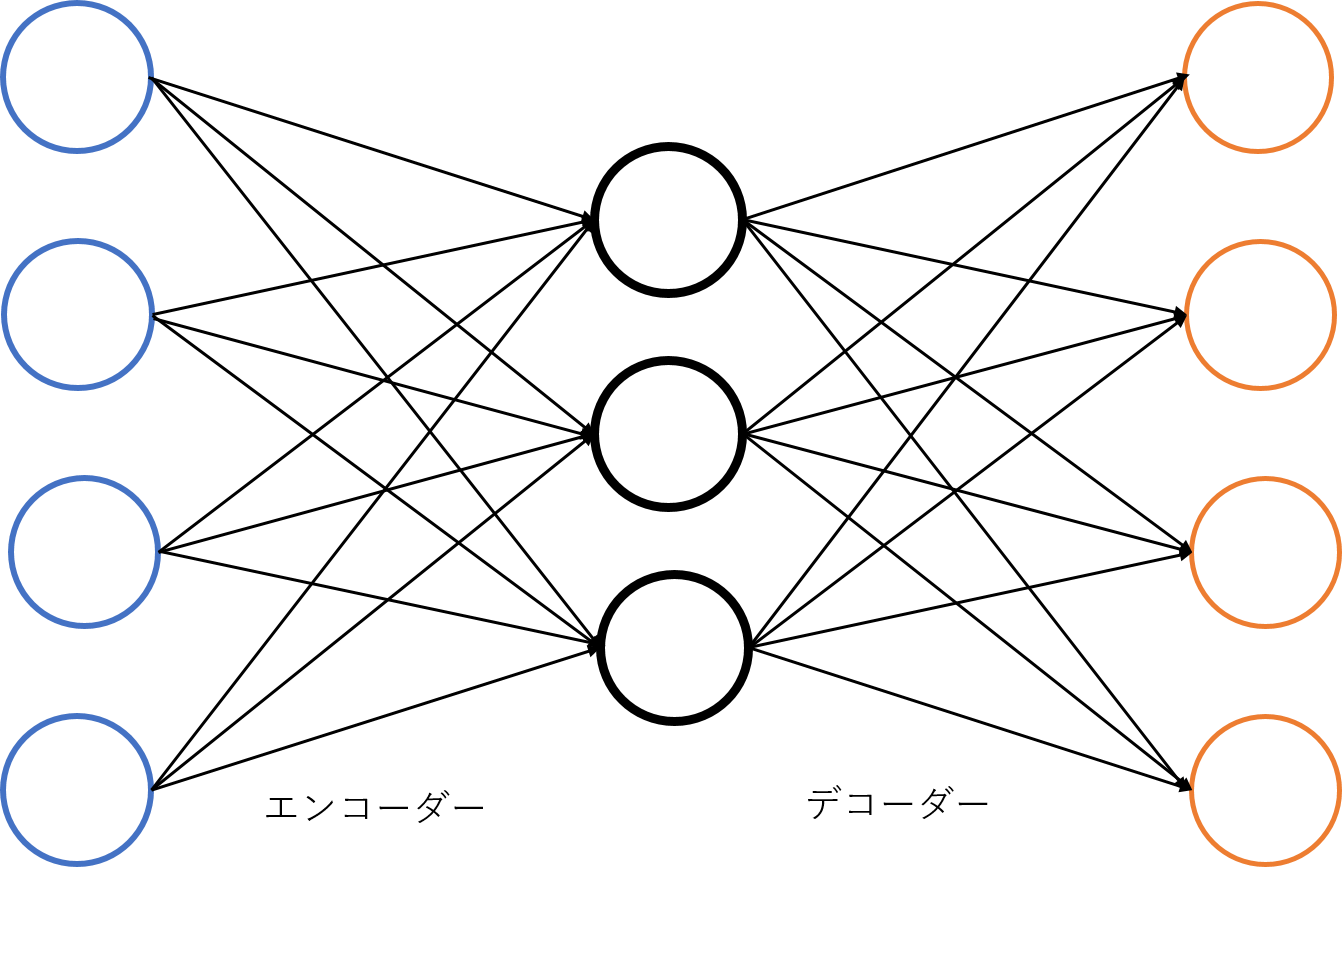
\includegraphics[clip, width=\linewidth]{AE_image.png}
          \hspace{0.2cm} [2]平均二乗誤差(実験1)
        \end{center}
      \end{minipage}


    \end{tabular}
    \caption{CNN(Adamで更新)}
     \label{fig:accuracy}
  \end{center}
\end{figure}
・DAE


・画像分類




\section{考察}

今回、自己符号化器を作成し、それを用いた画像識別を行った。
さまざまな構成で試したが、()が最も良い結果を生んだ。
ARA、CRPCRPAともに学習回数を重ねるとノイズなしでは高い再現性を実現した。しかしながらその学習にはとても時間がかかる。
また自己符号化器を使った事前学習での画像識別は前回やったMNISTデータで学習する時よりも初期の正解率が高く、平均二乗誤差も低い数値から始まり、結果として早く終息する傾向があるように思う。これは自己符号化で早くからパラメータの数値が良い値を示し、収束の加速につながったと思う。
しかし同じ構成のネットワークで学習をしてみるとノイズなしの方がより良い結果を示しているように思う。
これはノイズをつけた方がノイズにフィットするように学習が進むためだと思われる。

デノイジングに関してはこちらも学習回数というよりネットワーク構成が大きく影響することがわかる。
雑音除去はないものを周りのものを使って構成するという機能なのでかけてしまった歴史的な壁画や、これを文章に置き換え穴あき問題を解かせるなどに使えそうだなと作成しながら構想した。

今回はエンコーダーには畳み込み層を用いているが、デコーダ部分には畳み込みを持ちいらずアフィン層で拡張した
この構成が結果にどのような影響をあたえているかわからないのでdeconvolutionを用いた実装をしてみたいと思う。

コーディングしていく中でうまくネットワークを作るにはトライアンドエラーが必要不可けつだと感じた。
おそらく元とする学習データでもその構成は変わると思われる。
なのでコツは改変しやすいようクラスやオブジェクトで各モジュールをパッケージ化していくことだと思われる。
より柔軟性の高いコーディングを目指していきたい。




\clearpage

\begin{figure}[tb]
\begin{center}
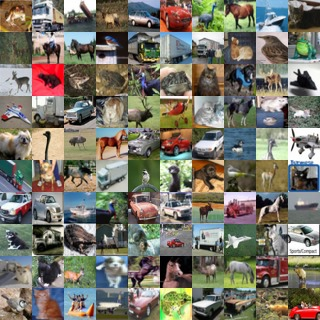
\includegraphics[width=\linewidth]{cyfer_ans.jpg}
\caption{学習データ} \label{fig:ae1}
\end{center}
\end{figure}

\begin{figure}[tb]
\begin{center}
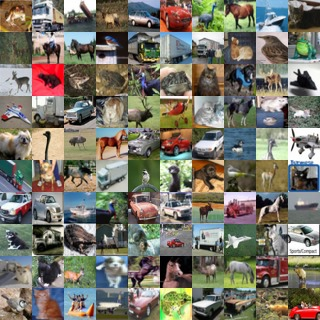
\includegraphics[width=\linewidth]{cyfer_ans.jpg}
\caption{学習データの復号結果(実験条件との対応がとれるようにすること): 学習回数=200回.平均二乗誤差=7.1715} \label{fig:ae}
\end{center}
\end{figure}

\end{document}
